\documentclass[11pt,reqno]{amsart}
\usepackage{amsmath,amssymb,amsthm}
\usepackage{booktabs}
\usepackage{array}
\usepackage{graphicx}
\usepackage{microtype}
\usepackage[margin=1.05in]{geometry}
\usepackage[hidelinks]{hyperref}

\newtheorem{theorem}{Theorem}[section]
\newtheorem{proposition}[theorem]{Proposition}
\newtheorem{lemma}[theorem]{Lemma}
\newtheorem{corollary}[theorem]{Corollary}
\theoremstyle{definition}
\newtheorem{definition}[theorem]{Definition}
\newtheorem{example}[theorem]{Example}
\newtheorem{question}[theorem]{Question}
\newtheorem{conjecture}[theorem]{Conjecture}
\theoremstyle{remark}
\newtheorem{remark}[theorem]{Remark}
\newtheorem{fact}[theorem]{Fact}

\emergencystretch=2em
\newcommand{\F}{\mathbb{F}}
\newcommand{\Z}{\mathbb{Z}}
\newcommand{\wt}{\operatorname{wt}}
\newcommand{\ord}{\operatorname{ord}}
\newcommand{\lcm}{\operatorname{lcm}}
\newcommand{\M}{\mathcal{M}}
\newcommand{\gen}[1]{\langle #1\rangle}

\title[Quantum Synchronizable Hybrid Codes]{Synchronizable Hybrid Codes from Cyclic Codes over $\F_q[v]/(v^3-v)$: Exact Misalignment Thresholds and the Limits of Component Fusion}
\author{Arun Kumar Yadav}
\address{School of Basic and Applied Sciences, K. R. Mangalam University, Gurugram 122103, India}
\email{arunyadav0317@gmail.com}
\subjclass[2020]{81P73, 94B15, 11T71}
\keywords{quantum synchronizable codes; hybrid quantum-classical codes; cyclic codes over finite rings; idempotent decomposition; block misalignment; order of a polynomial}

\begin{document}

\begin{abstract}
We study synchronizable hybrid codes built from cyclic codes over the reduced ring $R=\F_q[v]/(v^3-v)$, where $q$ is an odd prime and $\gcd(n,q)=1$. The Chinese remainder theorem gives $R\cong\F_q^3$, so a cyclic code over $R$ is a triple of cyclic codes over $\F_q$, and an interleaved lift places the three components on $3n$ qudits grouped into $n$ cells of three qudits. A block misalignment is a shift by a whole number of cells. Within an idealised model in which the marker syndrome is observed exactly, we prove that the collision differences of a component are precisely the multiples of $e=\ord_x(f)$, where $f$ is the quotient of the two generator polynomials, so the largest tolerable misalignment is $e-1$ cells; the known sufficient condition $a_l+a_r<e$ is therefore also necessary. For every dual-containing branch we show $\deg f\le e-1$, so the degree-type bound $\deg f-1$ is never sharp and can be arbitrarily far from the exact value. Three components fuse with period $\lcm(e_1,e_2,e_3)$, but the largest attainable period is $n$, already attained by a single component: fusion cannot enlarge the window, although it does allow the window to be sustained by components whose individual periods are small. When the marker carries classical symbols we give an exact collision criterion, prove that a collision at difference $\delta$ forces $|\delta|+y\ge\deg f$, and show that the window can be held by one component while the others transmit messages. A ternary example with underlying hybrid parameters $[[39,3:9,0,3]]_3$ transmits four ternary marker symbols over a twelve-cell window at a padded length of $75$ qudits. All numerical statements were re-derived by an independent exact-arithmetic implementation, including an exhaustive census of $20\,724$ dual-containing branches. No claim is made about noisy syndrome extraction.
\end{abstract}

\maketitle


\section{Introduction}\label{sec:introduction}

Quantum error-correcting codes protect encoded information against Pauli errors on the physical carriers; the stabilizer construction that underlies everything below is the CSS construction of Calderbank and Shor \cite{CalderbankShor1996} and Steane \cite{Steane1996}, and the simultaneous transmission of quantum and classical information in one block goes back to the operator-algebra framework of Kribs, Laflamme and Poulin \cite{KribsLaflammePoulin2005}. In a stream of encoded blocks they do not, by themselves, protect the receiver's knowledge of where each block begins. A frame displaced by a few positions causes the decoder to act on the wrong subset of carriers, and the resulting error is not a Pauli error of the encoded block but a mismatch between the physical positions and the coordinates the decoder assumes. Classical synchronizable codes address this problem with markers or comma-free constructions, an approach that goes back to Bose and Caldwell \cite{BoseCaldwell1967}. Such schemes rely on inspecting individual symbols, which is not directly possible for quantum data because measurement collapses the encoded state unless the measurement commutes with the encoded algebra; the synchronizable construction arranges precisely that, at the price of a marker that is measured only in a syndrome.


Fujiwara introduced quantum synchronizable codes (QSCs), in which recovery from block misalignment is built into the code algebra rather than obtained by inspecting the encoded state \cite{Fujiwara2013}. The construction starts from two classical cyclic codes $\mathcal C\subseteq\mathcal D$ of length $n$ over $\F_q$ with $\mathcal C^\perp\subseteq\mathcal C$, and uses the nested pair to attach a marker coset to a CSS-type code; the marker is measured only in the syndrome of $\mathcal C$, which leaves the encoded quantum information undisturbed. The magnitude of the tolerable misalignment is governed by the multiplicative order of the quotient polynomial $f=g_{\mathcal C}/g_{\mathcal D}$. Fujiwara's original sufficient condition $a_l+a_r<k_{\mathcal D}-k_{\mathcal C}$ was refined by Fujiwara, Tonchev and Wong to the order condition $a_l+a_r<\ord_x(f)$ \cite{FujiwaraTonchevWong2013}, which is the form used in essentially all later constructions: quadratic residue codes and their supercodes \cite{XieYuanFujiwara2014}, finite geometries \cite{FujiwaraVandendriessche2014}, cyclotomic classes \cite{LiZhuLiu2019,ShiYueHuang2021,LiZhu2022}, chain-containing $q$-ary codes \cite{XieYangYuan2016}, repeated-root and quasi-cyclic families \cite{LuoMa2018,DuMaLiu2023}, the $\lambda(u+v)|u-v$ construction \cite{DuMaLuoWang2020}, and further families with explicit distance or two new classes \cite{LuoMaLin2019,LiuKai2023} and BCH-type families \cite{SunEtAl2023}. Guenda, La Guardia and Gulliver gave an algebraic account of the framework \cite{GuendaEtAl2017}.


Two extensions of the basic problem are relevant here. The first replaces the field by a finite ring. Several authors have constructed QSCs from cyclic or constacyclic codes over rings, using Euclidean sums, chain rings, or rings of the form $\F_q+u\F_q$ \cite{LiuLiu2021,DaiLiu2022,LiuHuLiu2024}. Independently, the coding-theory literature has made extensive use of decomposable rings such as $\F_p[u]/(u^{k+1}-u)$ to build quantum codes from cyclic codes, with the Chinese remainder theorem reducing the problem to several field components \cite{DinhEtAl2021,DinhBagUpadhyay2021}. The second extension adds a classical message: hybrid quantum-classical codes carry quantum and classical information simultaneously, and Tansuwannont and Nemec have recently unified synchronizable codes, hybrid codes and subsystem codes, proving trade-offs between the number of correctable misalignments, the number of gauge qudits and the number of classical symbols \cite{TansuwannontNemec2026}.


This paper sits at the intersection of these two lines. We take the reduced ring $R=\F_q[v]/(v^3-v)$ with $q$ odd, so that $R\cong\F_q^3$ through three explicit primitive idempotents. A cyclic code over $R$ is then a triple $(\mathcal C_1,\mathcal C_2,\mathcal C_3)$ of cyclic codes over $\F_q$, and a chain $\mathcal C^\perp\subseteq\mathcal C\subseteq\mathcal D$ over $R$ is the same thing as three chains over $\F_q$. Placing the three components on disjoint coordinates of a block of $3n$ qudits, grouped into $n$ cells of three qudits, produces a hybrid code whose parameters are read off from the components. Because the three components share one physical frame, they also share one misalignment, which is measured in cells. This is the sense in which the ring is used: not as a source of new synchronization phenomena, but as a device that packages three synchronized components, with independent marker parameters, into a single block.


Our analysis is deliberately confined to an idealised observation model in which the marker syndrome is known exactly, either because the channel is noiseless or because the physical errors have already been corrected. Within that model the synchronization problem becomes a purely algebraic question about the map from the offset to the observed syndrome, and we answer it completely for a single component: the offsets that cannot be distinguished are exactly the multiples of $e=\ord_x(f)$, so the window is $e-1$ and the classical sufficient condition is also necessary. This much is implicit in the order-based literature, where $\ord_x(f)$ appears as a sufficient bound; making the converse explicit is what allows the subsequent comparison of designs, and we use it to settle three questions that the sufficient condition alone cannot answer.


First, how much is lost by the degree-type condition $a_l+a_r<\deg f$? For dual-containing branches nothing is gained by it, because dual containment forces $\deg f\le e-1$; the gap between the two criteria is therefore at least one cell for every branch and can be made arbitrarily large by taking $f$ to be an irreducible factor of a cyclotomic polynomial $\Phi_m$ with $m/\ord_m(q)$ large. This is a statement about the sharpness of a widely used bound, not a new construction.


Second, does using three components enlarge the attainable window? It does not. Since $e\mid n$ for every branch, the fused period $\lcm(e_1,e_2,e_3)$ never exceeds $n$, and a single component already attains $n$ whenever a nontrivial dual-containing branch exists. What fusion provides is a relaxation: a window of $n-1$ cells can be sustained by three components whose individual periods are far below $n$, which matters when no single branch of the required length is available or when the per-component code parameters must be kept small. We quantify this relaxation over a finite range and show that the relaxation factor is unbounded in general, at the price of a poor $X$-distance.


Third, how do classical messages interact with synchronization? Encoding a message in the marker residue restricts the set of admissible residues, and a collision then occurs exactly when a shifted residue lands back in the message family. We characterise this criterion exactly, prove the bound $|\delta|+y\ge\deg f$ that relates the collision distance $\delta$, the marker degree $y$ and the code parameter $\deg f$, and show that the work can be divided among the components: one component can hold the frame with an empty message while the others transmit. In the ternary example of Section 5.4 this yields four classical symbols over a twelve-cell window, out of the nine symbol slots that the underlying hybrid code offers.


The paper is organised as follows. Section 2 develops the algebra of $R$ and of cyclic codes over $R$, including the dual-containment criterion and the existence question for branches. Section 3 describes the interleaved construction, its parameters and its distance, and fixes the observation model. Section 4 proves the exact threshold for a single component, compares it with the degree bound, and analyses fusion. Section 5 treats message-carrying markers and the allocation of synchronization and message capacity. Section 6 reports the computational verification, Section 7 discusses limitations and Section 8 concludes. Appendix A records the sign convention in the collision criterion, and Appendix B extends the threshold theorem to marker residues that are not coprime to $f$.


A note on what is and is not claimed. The synchronization results are theorems about an idealised model with exact syndromes and offsets by whole cells; they say nothing about noisy syndrome extraction, about the propagation of physical errors into the offset estimate, or about fault-tolerant decoding. The distance statements are combinatorial and refer to the hybrid code's minimum distance in the usual sense. No claim of optimality is made for any construction: the thresholds are exact for the codes considered, but the codes themselves are not claimed to be optimal in any parameter regime.


\section{The coefficient ring and its cyclic codes}\label{sec:the-coefficient-ring-and-its-cyclic-codes}

Throughout, $q$ is an odd prime, $n\ge2$ satisfies $\gcd(n,q)=1$, and


\begin{equation}\label{eq:ring}
R=\F_q[v]/(v^3-v).
\end{equation}

For a polynomial $a$ of degree $d$ with $a(0)\neq0$ we write $a^*(x)=x^{d}a(1/x)$ for its reciprocal and call $a$ self-reciprocal when $a^*$ is a scalar multiple of $a$. All codes in this section have length $n$ and are cyclic.


\subsection{The idempotent decomposition}

\begin{proposition}\label{ring}
The polynomial $v^3-v=v(v-1)(v+1)$ has three distinct roots in $\F_q$, so the Chinese remainder theorem gives an isomorphism of $\F_q$-algebras $R\cong\F_q\times\F_q\times\F_q$. The corresponding primitive idempotents are

\begin{equation}\label{eq:idem}
\eta_1=1-v^2,\qquad \eta_2=\tfrac12(v^2+v),\qquad \eta_3=\tfrac12(v^2-v),
\end{equation}

and they satisfy $\eta_i^2=\eta_i$, $\eta_i\eta_j=0$ for $i\neq j$, $\eta_1+\eta_2+\eta_3=1$ and $v=\eta_2-\eta_3$. Every $r\in R$ has a unique expression $r=r_1\eta_1+r_2\eta_2+r_3\eta_3$ with $r_i\in\F_q$.
\end{proposition}

\begin{remark}\label{char}
The hypothesis that $q$ is odd is essential for the formula @eq:idem, not for the decomposition as such. Over $\F_2$ one has $v^3-v=v(v+1)^2$, the ring is not reduced, and $\tfrac12(v^2\pm v)$ is undefined. Nothing in Sections 2--5 uses primality of $q$; the restriction to prime fields is made because the enumerations of Section 6 were carried out over prime fields. The case $q=3$ is included, with $\tfrac12=2$: then $\eta_2=2v^2+2v$ and $\eta_3=2v^2+v$, and indeed $\eta_2+\eta_3=v^2$ and $\eta_2-\eta_3=v$.
\end{remark}

A cyclic code of length $n$ over $R$ is an ideal of $R[x]/(x^n-1)$. Since $R[x]/(x^n-1)\cong\bigoplus_{i=1}^{3}\F_q[x]/(x^n-1)$, every such ideal has the form


\begin{equation}\label{eq:decomp}
C=\eta_1C_1\oplus\eta_2C_2\oplus\eta_3C_3,\qquad C_i=\gen{g_i}\subseteq\F_q[x]/(x^n-1),\quad g_i\mid x^n-1,
\end{equation}

and $C=\gen{\eta_1g_1+\eta_2g_2+\eta_3g_3}$. We call $C_i$ the $i$-th component of $C$. On $R^n$ we use the Euclidean form $\langle u,w\rangle=\sum_t u_tw_t\in R$, whose values lie in $R$ rather than in $\F_q$; orthogonality is therefore tested in each component separately, as the next proposition records.


\begin{proposition}\label{components}
Let $k_i=\dim_{\F_q}C_i$. Then $\dim_{\F_q}C=k_1+k_2+k_3$ and $|C|=q^{k_1+k_2+k_3}$. The code $C$ is a free $R$-module if and only if $k_1=k_2=k_3$. Moreover

\begin{equation}\label{eq:dualcomp}
C^\perp=\eta_1C_1^\perp\oplus\eta_2C_2^\perp\oplus\eta_3C_3^\perp,\qquad\text{so}\qquad C^\perp\subseteq C\iff C_i^\perp\subseteq C_i\ \text{for } i=1,2,3.
\end{equation}
\end{proposition}

\begin{remark}\label{rank}
All statements below are phrased in terms of $\dim_{\F_q}C=\sum_ik_i$ and of the component codes; no $R$-rank is used. Non-free codes are admissible: for $q=5$ and $n=4$ the component dimensions $(4,3,4)$ give $|C|=5^{11}$.
\end{remark}

\subsection{Dual containment}

For a divisor $g$ of $x^n-1$ over $\F_q$ put $h=(x^n-1)/g$. It is standard that $\gen{g}^\perp=\gen{h^*}$; the next lemma records the resulting criterion in the three equivalent forms used below.


\begin{lemma}\label{dc}
Let $C=\gen{g}$ with $g\mid x^n-1$. Then $C^\perp\subseteq C$ if and only if $g\mid h^*$, equivalently $g g^*\mid x^n-1$, equivalently no irreducible factor $p$ of $g$ has $p^*$ (up to a scalar) dividing $g$. In particular $x-1\nmid g$ whenever $C^\perp\subseteq C$ and $C\neq\{0\}$.
\end{lemma}

The last assertion uses that $x-1$ is self-reciprocal and that $x-1$ divides $x^n-1$ exactly once when $\gcd(n,q)=1$. The criterion itself is classical; we use it only to decide which branches exist.


Which $(q,n)$ admit a nontrivial dual-containing code is decided by the position of $-1$ in the group generated by $q$. The following statement is the dual-containment counterpart of Massey's characterisation of reversible cyclic codes \cite{Massey1964} and of the complementary-dual condition of Yang and Massey \cite{YangMassey1994}; we record it because it determines the range of the construction.


\begin{lemma}\label{selfrecip}
Let $d\mid n$ and let $p$ be an irreducible factor of the cyclotomic polynomial $\Phi_d$ over $\F_q$. Then $p$ is self-reciprocal if and only if $-1\in\gen{q}\subseteq(\Z/d\Z)^*$. In particular, if $-1\notin\gen{q}\subseteq(\Z/n\Z)^*$ then every irreducible factor of $\Phi_n$ is non-self-reciprocal.
\end{lemma}

\begin{theorem}\label{existence}
There is a cyclic code $C$ of length $n$ over $\F_q$ with $\{0\}\neq C^\perp\subseteq C\subsetneq\F_q^n$ if and only if $-1\notin\gen{q}\subseteq(\Z/n\Z)^*$.
\end{theorem}

\begin{example}\label{nogo}
For $(q,n)=(3,10)$ and $(7,10)$ one has $\gen{3}=\gen{7}=\{1,3,7,9\}\ni-1$ in $(\Z/10\Z)^*$. Hence no nontrivial dual-containing cyclic code of length $10$ exists over $\F_3$ or over $\F_7$, and no synchronizable code of the type considered here, with or without a ring structure, exists for these parameters.
\end{example}

Two consequences of Theorem \ref{existence} are used repeatedly. First, the existence question for the ring code is exactly the existence question for a single field component, because Proposition \ref{components} reduces dual containment to the three components. Second, whenever branches exist, one of them has order $n$; this is Lemma \ref{periodn} in Section 4 and it is what caps the achievable window.


\section{The interleaved construction}\label{sec:the-interleaved-construction}

\subsection{Layout and offset model}

The physical system consists of $3n$ qudits of dimension $q$, grouped into $n$ cells of three qudits. Position $3t+i-1$, with $0\le t\le n-1$ and $i=1,2,3$, carries the $i$-th component of the ring symbol $c_t=c_t^{(1)}\eta_1+c_t^{(2)}\eta_2+c_t^{(3)}\eta_3$, as in Figure~\ref{fig:lift}. A frame misalignment is a cyclic shift of the ring word by $\alpha\in\Z_n$ cells, that is, a shift of the $3n$ qudits by $3\alpha$ positions. The offset is common to the three components because it is a property of the block structure and not of a component. Shifts by one or two qudits, which would move the components relative to one another, lie outside the model; this is the main structural restriction imposed by the interleaving, and we return to it in Section 7. A block padded by $a_l$ cells on the left and $a_r$ cells on the right occupies $3(n+a_l+a_r)$ qudits, so padding is counted in cells as well.


\begin{figure}[t]
\centering
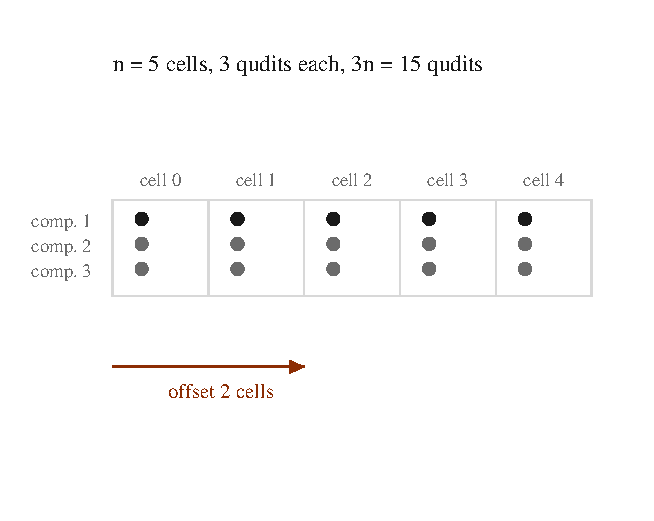
\includegraphics[width=0.8\linewidth]{figures/fig_lift.pdf}
\caption{The interleaved lift for $n=5$. Each cell holds one qudit of each component; a frame offset of $\alpha$ cells shifts all three components by the same number of positions.\label{fig:lift}}
\end{figure}

\subsection{Parameters}

Fix a chain $C^\perp\subseteq C\subseteq D$ of $R$-cyclic codes of length $n$. By Proposition \ref{components} this is the same as three chains $C_i^\perp\subseteq C_i\subseteq D_i$ of cyclic codes over $\F_q$ with generator polynomials $g_{C_i}$ and $g_{D_i}$. A component with $C_i\subsetneq D_i$ is called a \emph{branch}; a component with $C_i=D_i$ is \emph{inactive}. For a branch we write


\begin{equation}\label{eq:fi}
f_i=\frac{g_{C_i}}{g_{D_i}},\qquad e_i=\ord_x(f_i),\qquad \deg f_i=k_{D,i}-k_{C,i},
\end{equation}

where $\ord_x(f)$ denotes the multiplicative order of $x$ in the finite ring $\F_q[x]/(f)$, that is, the least $e\ge1$ with $x^e\equiv1\pmod f$. The order is defined because $f(0)\neq0$ for a proper divisor of $x^n-1$. For an inactive component we set $f_i=1$ and $e_i=1$; its marker syndrome is constant and imposes no condition on the offset. We write $[[N,K:M,R_g,d]]_q$ for a code on $N$ qudits with $K$ logical qudits, $M$ classical $q$-ary symbols, $R_g$ gauge qudits and distance $d$, following the parameter roles of \cite{TansuwannontNemec2026}.


\begin{proposition}\label{params}
The interleaved lift of the chain $C^\perp\subseteq C\subseteq D$ is a hybrid code with parameters $[[N,K:M,0,d]]_q$ where

\begin{equation}\label{eq:params}
N=3n,\qquad K=\sum_{i=1}^{3}(2k_{C,i}-n),\qquad M=\sum_{i=1}^{3}(k_{D,i}-k_{C,i}),\qquad d=\min(d_X,d_Z),
\end{equation}

and

\begin{equation}\label{eq:dist}
d_X=\min_i\ \min\wt(D_i\setminus C_i^\perp),\qquad d_Z=\min_i\ \min\wt(C_i\setminus C_i^\perp).
\end{equation}

In particular $d\ge\min_i d(D_i)$ and $d\ge\min_i d(C_i)$, where $d(\cdot)$ is the minimum distance of the classical code.
\end{proposition}

\textbf{Proof.} Work first with a single component and drop the index. The operators $X(a)$ and $Z(b)$ with $a,b\in C^\perp$ commute, since $X(a)Z(b)=\omega^{a\cdot b}Z(b)X(a)$ with $\omega=e^{2\pi i/q}$ and $a\cdot b=0$ because $a,b\in C^\perp\subseteq(C^\perp)^\perp=C$. They therefore generate a stabilizer group of order $q^{2(n-k_C)}$ and the number of logical qudits is $n-2(n-k_C)=2k_C-n$. The transmitted word is $|\psi+g\rangle$ with $\psi$ a superposition of codewords of $C$ and $g\in D$ the classical label. Measuring the $Z$-syndrome with respect to $C^\perp$, that is the eigenvalues of $Z(v)$ for a basis of $v\in C^\perp$, returns $v\cdot(c+g)=v\cdot g$ for every $c\in C$, so the outcome is independent of the codeword and the measurement leaves the superposition intact; it equals the class of $g$ modulo $(C^\perp)^\perp=C$. Hence the classical label is an element of $D/C$ and there are $q^{k_D-k_C}$ of them. An $X$-type error $X(e)$ is a stabilizer when $e\in C^\perp$; when $e\in C\setminus C^\perp$ it leaves the label in its class but acts as a nontrivial logical $X$; when $e\in D\setminus C$ it moves the label to another valid class, and the receiver cannot tell this from a different message; and when $e\notin D$ the observed class is not a valid message and the error is flagged. The undetected and harmful $X$-type errors are therefore exactly the elements of $D\setminus C^\perp$, which gives $d_X$. For a $Z$-type error, $Z(v)$ commutes with the label measurement if and only if $v\in C$, and among those it is trivial on the code space if and only if $v\in C^\perp$, which gives $d_Z$. An operator mixing the two types has weight at least the larger of the weights of its parts and its nontrivial part is of one of the two kinds already counted, so the minimum is $\min(d_X,d_Z)$. The lift places the three components on disjoint coordinates, so the stabilizer groups multiply, $K$ and $M$ add, and the distance is the minimum over the components. No gauge qudits occur because the construction is symmetric in $X$ and $Z$; the general asymmetric case is described in Remark \ref{subsystem}. The final bounds follow from $D_i\setminus C_i^\perp\subseteq D_i\setminus\{0\}$ and $C_i\setminus C_i^\perp\subseteq C_i\setminus\{0\}$. $\square$


The parameter count should be read with care. $M$ counts classical symbol slots, not synchronized ones: Section 5 shows that part of this capacity must be spent on marker degrees of freedom if a window is required.


\begin{remark}\label{properD}
For a branch $C^\perp\subseteq C\subsetneq D$, the condition $\min\wt(D\setminus C^\perp)\ge2$, that is $d_X\ge2$, is equivalent to $D\neq\F_q^n$. Indeed, a cyclic code containing a word of weight one contains all of its cyclic shifts, hence all unit vectors, hence is the full space. Conversely, if $D=\F_q^n$ then no unit vector lies in $C^\perp$, since cyclicity would force $C^\perp=\F_q^n$ and $C=\{0\}$, contradicting dual containment. This equivalence concerns the threshold $2$ only; it says nothing about larger distance requirements.
\end{remark}

\subsection{The observation model}

In the construction the transmitted word is $|\psi+g\rangle$, where $\psi$ is the encoded quantum state in $C$ and $g\in D$ is the marker codeword. By the proof of Proposition \ref{params} this same $g$ is the classical label, so the marker and the classical symbol are one object rather than two: the $M$ symbol slots of the hybrid code are exactly the $M$ coordinates of the marker, and the receiver obtains them by measuring the $Z$-syndrome with respect to $C^\perp$. The block is then padded cyclically and the receiver measures, on the $n$ positions it takes to be the block, the syndrome of the marker with respect to $g_C$. If the true frame is shifted by $\alpha$, the measured syndrome is the class of $x^\alpha g$ modulo $g_C$. Writing $g=g_D\beta$, the marker is described by its \emph{residue} $\beta$ modulo $f$; the natural choice is $\beta=1$, that is $g=g_D$. For the ring code the receiver observes the triple of component syndromes


\begin{equation}\label{eq:sigma}
\Sigma(\alpha)=\bigl(x^\alpha g_{D_1}\bmod g_{C_1},\ x^\alpha g_{D_2}\bmod g_{C_2},\ x^\alpha g_{D_3}\bmod g_{C_3}\bigr).
\end{equation}

Suppose the offset is known to lie in $[-a_r,a_l]$ with $a_l,a_r\ge0$ and put $W=a_l+a_r\le n-1$. The offset is \emph{recoverable} if $\alpha\mapsto\Sigma(\alpha)$ is injective on $[-a_r,a_l]$, that is, if no difference $\delta=\alpha-\alpha'$ with $1\le|\delta|\le W$ is a \emph{collision} in the sense $\Sigma(\alpha)=\Sigma(\alpha')$. The largest $W$ for which this holds is the \emph{window} of the code. Because $\Sigma$ is defined on $\Z_n$, the window never exceeds $n-1$.


The following assumptions delimit the analysis; they are stated once and used throughout Sections 4 and 5.


(A1) Offsets are whole cells and satisfy $W\le n-1$. (A2) The marker syndrome @eq:sigma is known exactly. This is the case if the channel is noiseless, or if the physical errors have been corrected before the offset is estimated. (A3) The receiver knows $g_{C_i}$, $g_{D_i}$ and the message family in use. (A4) Physical Pauli errors are the object of the distance statement of Proposition \ref{params}; they are not modelled jointly with the offset estimate. (A5) There is no qudit loss, insertion or deletion, and the syndrome-extraction circuit is not itself noisy.


Under (A1)--(A5) the synchronization problem is exactly the injectivity question for @eq:sigma, and the results of Sections 4 and 5 are theorems about that question. They do not assert that a physical receiver subject to the failure modes of (A2) will synchronize; that requires a separate analysis of syndrome noise and of the coupling between physical errors and the offset estimate. Figure~\ref{fig:flow} summarises the design pipeline and marks the point at which the idealisation enters.


\begin{figure}[t]
\centering
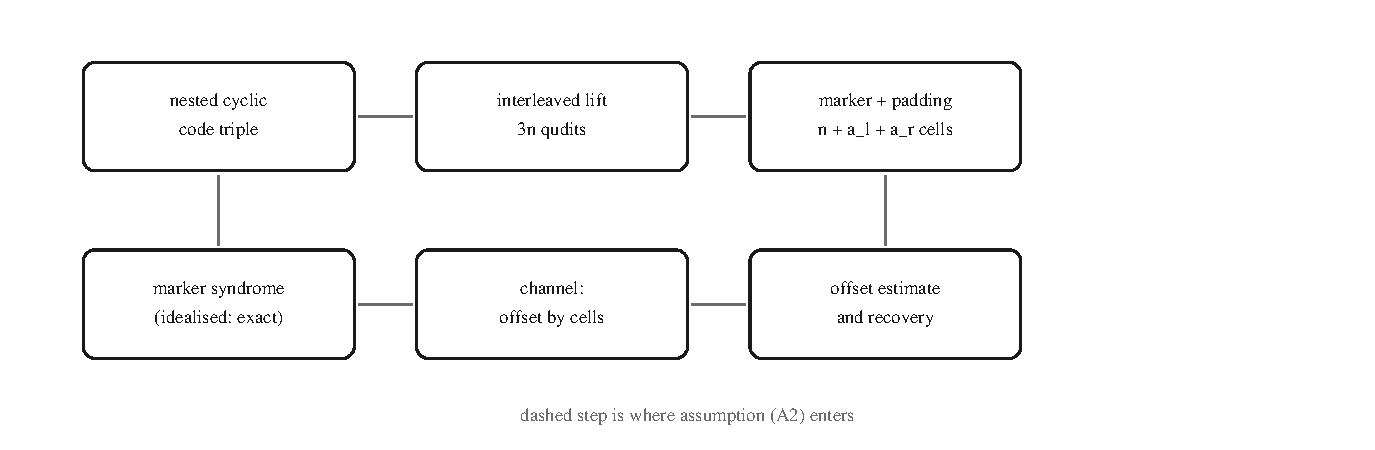
\includegraphics[width=0.8\linewidth]{figures/fig_flow.pdf}
\caption{Construction and decoding pipeline. The shaded box marks the step that the idealised model (A2) replaces by an exact observation; the analysis in this paper covers the algebraic parts and the distance statement, not the noisy extraction.\label{fig:flow}}
\end{figure}

\section{Exact misalignment thresholds}\label{sec:exact-misalignment-thresholds}

\subsection{A single component}

Fix one component and drop the index. Let $C\subsetneq D$ be cyclic codes of length $n$ over $\F_q$, let $f=g_C/g_D$ and $e=\ord_x(f)$. Neither the collision lemma nor Theorem \ref{sharp} uses the dual-containment condition; they are statements about nested cyclic codes.


\begin{lemma}\label{collision}
Let $g=g_D\beta$ and $g'=g_D\beta'$ be marker codewords with residues $\beta,\beta'$ modulo $f$. Then $x^\alpha g\equiv x^{\alpha'}g'\pmod{g_C}$ if and only if

\begin{equation}\label{eq:collision}
f\mid x^\delta\beta-\beta',\qquad \delta=\alpha-\alpha'.
\end{equation}
\end{lemma}

\textbf{Proof.} The congruence means $g_C\mid x^{\alpha'}(x^\delta g_D\beta-g_D\beta')$ with $x^\delta$ read modulo $x^n-1$. Since $g_C\mid x^n-1$ and $x$ is invertible modulo $x^n-1$, this is equivalent to $g_C\mid g_D(x^\delta\beta-\beta')$, and division by $g_D$ gives @eq:collision. $\square$


\begin{theorem}\label{sharp}
Let the marker residue $\beta$ be coprime to $f$, for instance $\beta=1$. A difference $\delta$ is a collision if and only if $e\mid\delta$. Consequently the syndrome map is injective on $[-a_r,a_l]$ if and only if $a_l+a_r\le e-1$, and the window equals $e-1$.
\end{theorem}

\textbf{Proof.} By Lemma \ref{collision}, $\delta$ is a collision if and only if $f\mid\beta(x^\delta-1)$, which by $\gcd(\beta,f)=1$ is equivalent to $f\mid x^\delta-1$, that is $e\mid\delta$. The differences occurring in $[-a_r,a_l]$ are those with $1\le|\delta|\le a_l+a_r$, and none of them is a multiple of $e$ exactly when $a_l+a_r<e$. $\square$


The sufficiency of $a_l+a_r<e$ is the order criterion of \cite{FujiwaraTonchevWong2013,XieYangYuan2016,LuoMa2018}; Theorem \ref{sharp} adds that no larger window is possible in the ideal model and identifies the complete collision set. This is a short argument, but it changes the status of the order condition from a bound to an exact value, and the rest of the paper uses that change: comparisons between designs, and the negative results on fusion, are statements about the exact value.


Two immediate consequences deserve recording. First, since $f\mid x^n-1$,


\begin{equation}\label{eq:edivn}
e\mid n\quad\text{for every branch,}
\end{equation}

so the window is at most $n-1$ for every choice of nested pair. Second, the same argument applied to an arbitrary marker family shows that the multiples of $e$ are always collisions, whatever the marker encodes; this yields a uniform ceiling that is used in Section 5.


\begin{corollary}\label{ceiling}
For every marker residue and every marker family, the window of a branch satisfies $W\le e-1$. In particular the window of a ring code whose active components have periods $e_1,e_2,e_3$ satisfies $W\le\lcm(e_1,e_2,e_3)-1\le n-1$.
\end{corollary}

The proof is the observation that $x^e\equiv1\pmod f$, so a shift by $e$ cells returns every marker to itself and is therefore a collision. Appendix B removes the coprimality hypothesis of Theorem \ref{sharp} and shows that the collision set is then the set of multiples of $\ord_x(f/\gcd(f,\beta))$, so a marker that shares a factor with $f$ loses part of the window in a way that is again computable exactly.


\subsection{The degree bound and its sharpness}

Fujiwara's original construction certifies a window from the codimension, and the hybrid framework of \cite{TansuwannontNemec2026} uses the same degree-type condition. The following comparison is therefore relevant to published statements rather than only to the present construction.


\begin{proposition}\label{degree}
If $a_l+a_r<\deg f=k_D-k_C$, the syndrome map is injective on $[-a_r,a_l]$.
\end{proposition}

\textbf{Proof.} Since $f\mid x^e-1$ we have $\deg f\le e$, and the claim follows from Theorem \ref{sharp}. $\square$


\begin{proposition}\label{gap}
If $C^\perp\subseteq C\subsetneq D$, then $\deg f\le e-1$. Hence the exact window $e-1$ is always at least $\deg f$, while the degree criterion certifies only $\deg f-1$.
\end{proposition}

\textbf{Proof.} By Lemma \ref{dc}, $x-1\nmid g_C$ and therefore $x-1\nmid f$. Both $f$ and $x-1$ divide the squarefree polynomial $x^e-1$ and are coprime, so $f(x-1)\mid x^e-1$ and $\deg f\le e-1$. $\square$


The gap is not a small constant. Table~\ref{tab:single} lists four branches with $d_X\ge2$; in the first row the exact window is twelve cells while the degree criterion certifies two. The ratio can be made arbitrarily large: if $f$ is an irreducible factor of $\Phi_m$ over $\F_q$, then $\deg f=\ord_m(q)$ and $e=m$, so $e/\deg f=m/\ord_m(q)$ is unbounded as $m$ varies over primes for which $\ord_m(q)$ stays small. The degree criterion is also sharp in general, outside the dual-containing setting: for $f=x-1$ one has $\deg f=e=1$ and both criteria give the empty window, so Proposition \ref{gap} is a consequence of dual containment and not of the degree count alone.


\begin{table}[t]
\centering
\caption{Branches $C^\perp\subseteq C\subsetneq D\subsetneq\F_q^n$: exact window $e-1$ against the degree bound $\deg f-1$. All entries were recomputed by exhaustive enumeration of the two cyclic codes.\label{tab:single}}
\small
\begin{tabular}{rlllcccccc}
\toprule
$q$ & $n$ & $g_C$ & $g_D$ & $(k_C,k_D)$ & $\deg f$ & $e$ & window & degree bound & $(d_Z,d_X)$ \\
3 & 13 & $1+x^2+x^5+x^6$ & $2+x+x^2+x^3$ & $(7,10)$ & 3 & 13 & 12 & 2 & $(4,3)$ \\
5 & 8 & $1+2x+3x^2+x^3$ & $3+x$ & $(5,7)$ & 2 & 8 & 7 & 1 & $(3,2)$ \\
7 & 6 & $6+2x+x^2$ & $5+x$ & $(4,5)$ & 1 & 6 & 5 & 0 & $(3,2)$ \\
11 & 5 & $3+9x+x^2$ & $2+x$ & $(3,4)$ & 1 & 5 & 4 & 0 & $(3,2)$ \\
\bottomrule
\end{tabular}

\smallskip
\parbox{\linewidth}{\footnotesize $d_Z=\min\wt(C\setminus C^\perp)$ and $d_X=\min\wt(D\setminus C^\perp)$ are obtained by enumerating all codewords; the window is $e-1$ by Theorem \ref{sharp}. Coefficients are listed in increasing powers of $x$.}
\end{table}

\subsection{Fusion of three components}

\begin{theorem}\label{fused}
For each active component let $e_i=\ord_x(f_i)$ and let the marker residue be coprime to $f_i$; for an inactive component set $f_i=1$ and $e_i=1$. Then the joint map $\alpha\mapsto\Sigma(\alpha)$ is injective on $[-a_r,a_l]$ if and only if $a_l+a_r\le e_R-1$, where $e_R=\lcm(e_1,e_2,e_3)$; the joint collisions are the multiples of $e_R$. In particular $\max_ie_i\le e_R\le n$.
\end{theorem}

\textbf{Proof.} A difference is a joint collision if and only if it is a collision in every component, that is, if and only if $e_i\mid\delta$ for all $i$ by Theorem \ref{sharp} for the active components and by constancy of the syndrome for the inactive ones. This is the condition $e_R\mid\delta$. The inequalities follow from $e_i\mid e_R$ and @eq:edivn. $\square$


Thus one triple may well gain from fusion: components with periods $(3,4,5)$ fuse to $60$, and Table~\ref{tab:relax} lists the triples of that kind with the largest ratio between the fused period and the largest component period. The question is whether fusion raises the \emph{best achievable} window, and the answer is negative.


\begin{lemma}\label{periodn}
Let $E(q,n)$ be the set of periods $\ord_x(f)$ of branches $C^\perp\subseteq C\subsetneq D$ of length $n$ over $\F_q$. Then $E(q,n)\neq\emptyset$ if and only if $-1\notin\gen{q}\subseteq(\Z/n\Z)^*$, and in that case $n\in E(q,n)$.
\end{lemma}

\textbf{Proof.} If $-1\in\gen{q}$ there is no branch by Theorem \ref{existence}. Otherwise let $p$ be an irreducible factor of $\Phi_n$. By Lemma \ref{selfrecip} it is not self-reciprocal, so $C=\gen{p}$ is dual-containing by Lemma \ref{dc}. With $D=\F_q^n$ one gets $f=p$, whose roots are primitive $n$-th roots of unity, hence $\ord_x(p)=n$. $\square$


\begin{theorem}\label{nogain}
If $-1\in\gen{q}\subseteq(\Z/n\Z)^*$, no synchronizable code of the above type exists over $\F_q$ or over $R$. Otherwise

\begin{equation}\label{eq:nogain}
\max_{\text{triples}}\lcm(e_1,e_2,e_3)=\max E(q,n)=n,
\end{equation}

so the largest window of a ring code of length $n$ is $n-1$ and is already attained by a single component. The same holds for any number of components.
\end{theorem}

\textbf{Proof.} The first statement combines Theorem \ref{existence} with Proposition \ref{components}. By @eq:edivn every $e_i$ divides $n$, so $\lcm(e_1,e_2,e_3)\le n$; by Lemma \ref{periodn} $n\in E(q,n)$, and the triple $(n,n,n)$ attains the bound. The argument does not refer to the number of components. $\square$


The ring's contribution is therefore not the window itself but the freedom to distribute it. This is worth stating precisely, because a natural reading of "three components fused by an lcm" suggests a gain that Theorem \ref{nogain} rules out.


\begin{remark}\label{relax}
What the ring provides is a \emph{relaxation}: the maximal period $n$ can be obtained from three components whose individual periods $m_1,m_2,m_3$ are much smaller, provided $\lcm(m_1,m_2,m_3)=n$. For $n\mid q-1$ this is realised by linear branches $C_i=\gen{x-a_i}\subsetneq\F_q^n$ with $a_i\in\F_q^*$ of order $m_i$. For a reproducible finite enumeration take every odd prime $q\le101$ and every $n\ge3$ dividing $q-1$, enumerate the sorted divisor triples $3\le m_1\le m_2\le m_3$ with $m_i\mid n$ and $\lcm(m_1,m_2,m_3)=n$, and for each $(q,n)$ minimise the largest order, breaking ties lexicographically. This gives $118$ pairs, of which $38$ have relaxation factor $n/\max_im_i>1$; the maximum in this range is $12$, attained at $(q,n)=(61,60)$ with orders $(3,4,5)$. The bound is not universal: the orders $(5,6,7)$ at $(211,210)$ give factor $30$ and $(5,7,8)$ at $(281,280)$ give factor $35$. In general, for pairwise coprime $a,b,c\ge3$ choose a prime $q\equiv1\pmod{abc}$, whose existence is Dirichlet's theorem, and put $n=a b c$; linear branches of orders $(a,b,c)$ then have factor $a b c/\max(a,b,c)$, and the choice $(a,b,c)=(t,t+1,2t+1)$ makes this $t(t+1)$. These linear families have $d_X=1$ and therefore do not improve the Pauli-error distance.
\end{remark}

\begin{question}\label{distance}
Does $\max_{\text{triples}}\lcm(e_1,e_2,e_3)=n$ persist when $\min\wt(D_i\setminus C_i^\perp)\ge t$ is required on every branch, for $t\ge4$? For $t=2$, equivalently proper $D_i$ by Remark \ref{properD}, it holds in all $27$ admissible pairs of Table~\ref{tab:dconstr}, and at $(q,n)=(3,13)$ the branch of Example \ref{flagship} is a witness with $t=3$. Larger $t$ was beyond our search, and we do not conjecture an answer.
\end{question}

\section{Message-carrying markers}\label{sec:message-carrying-markers}

\subsection{Marker families}

A marker that carries classical information has a residue restricted to a message family. Fix a branch with $f=g_C/g_D$, $e=\ord_x(f)$ and an integer $y$ with $0\le y\le\deg f-1$, and put


\begin{equation}\label{eq:My}
\M_y=\{1+b_1x+\cdots+b_yx^y:\ b_1,\dots,b_y\in\F_q\}\subseteq\F_q[x]/(f),\qquad |\M_y|=q^y.
\end{equation}

The condition $b_0=1$ normalises the family: every nonzero residue class modulo $f$ has a unique scalar multiple with constant term $1$, so $\M_y$ selects one representative from each of $q^y$ classes rather than a linear subspace. This is what makes the family closed under the comparison of two messages and keeps the zero residue out of the message set for $y<\deg f$.


\begin{lemma}\label{marker}
Let $0\le y$ and let $\M_y$ be as in @eq:My. If $y\le\deg f$, distinct elements of $\M_y$ have distinct residues modulo $f$; for $y=\deg f$ the reduction map $\M_{\deg f}\to\F_q[x]/(f)$ is a bijection. If $y\ge\deg f+1$, two distinct elements of $\M_y$ have the same residue.
\end{lemma}

\textbf{Proof.} If $b\neq b'$ in $\M_y$ had $b\equiv b'\pmod f$, then $u=b-b'$ would be a nonzero polynomial of degree at most $y$ divisible by $f$, so $\deg f\le y$; and $u(0)=0$. For $y<\deg f$ this is impossible. For $y=\deg f$ the only possibility would be $u=c f$ with $c\neq0$, which has $u(0)=c f(0)\neq0$, again impossible; the map is then injective between sets of size $q^{\deg f}$, hence bijective. For $y\ge\deg f+1$, $b=1+x f$ and $b'=1$ are distinct elements of $\M_y$ with equal residues. $\square$


The boundary case $y=\deg f$ is worth isolating, because it is the point at which the message family fills the whole quotient ring and the zero class enters: $\M_{\deg f}$ is a complete set of representatives of $\F_q[x]/(f)$, so for every offset difference $\delta$ and every $b\in\M_{\deg f}$ the residue of $x^\delta b$ is again an admissible message, and every nonzero $\delta$ is a collision. A positive window therefore requires $y\le\deg f-1$ in every component that is used for messages.


\subsection{The collision criterion}

\begin{theorem}\label{hybrid}
Fix a branch with $f$, $e$ and a marker family $\M_y$ with $0\le y\le\deg f-1$, and let $\Delta\subseteq\Z_n\setminus\{0\}$ be the set of collision differences. 1. A difference $\delta\neq0$ lies in $\Delta$ if and only if $x^\delta\M_y\cap\M_y\neq\emptyset$ modulo $f$, that is, if and only if $x^\delta b\bmod f\in\M_y$ for some $b\in\M_y$. 2. If $\delta\in\Delta$ then $|\delta|+y\ge\deg f$. Consequently $a_l+a_r\le\deg f-y-1$ guarantees injectivity, without knowledge of $e$. 3. For $y=0$ the collision set is the set of multiples of $e$ and the window is $e-1$.
\end{theorem}

\textbf{Proof.} (1) A collision means $f\mid x^\delta b-b'$ for some $b,b'\in\M_y$, which is the same as $x^\delta b\bmod f=b'$. (2) For $\delta\ge1$ the polynomial $u=x^\delta b-b'$ is nonzero: $b$ has constant term $1$, so $x^\delta b$ has constant term $0$ and $u(0)=-1\neq0$. Since $f\mid u$ and $\deg u\le\delta+y$, we get $\deg f\le\delta+y$. For $\delta\le-1$, multiply the congruence by the unit $x^{|\delta|}$ modulo $f$ and exchange the roles of $b$ and $b'$. (3) With $\M_0=\{1\}$ this is Theorem \ref{sharp}. $\square$


Part (2) is a bound, not a value, and the difference matters. When $e>\deg f$ the exact window can exceed the guarantee, as Table~\ref{tab:hybrid} shows in the second row, where the exact window is two cells and the guarantee one. When the guarantee is attained it is attained exactly at $\delta+y=\deg f$, as in the third and fifth rows. Both behaviours occur for the same branch as $y$ varies, so neither can be inferred from $\deg f$ alone.


\begin{table}[t]
\centering
\caption{Collision sets for message-carrying markers with $0\le y\le\deg f-1$; the last column is the guarantee $\deg f-y-1$ of Theorem \ref{hybrid}(2).\label{tab:hybrid}}
\small
\begin{tabular}{rrlccccclc}
\toprule
$q$ & $n$ & $f$ & $\deg f$ & $e$ & $y$ & $|\M_y|$ & collisions $\delta\in[1,n-1]$ & window & guarantee \\
3 & 13 & $2+2x+x^3$ & 3 & 13 & 0 & 1 & none & 12 & 2 \\
3 & 13 & $2+2x+x^3$ & 3 & 13 & 1 & 3 & $\{3,10\}$ & 2 & 1 \\
3 & 13 & $2+2x+x^3$ & 3 & 13 & 2 & 9 & all & 0 & 0 \\
5 & 8 & $2+x^2$ & 2 & 8 & 0 & 1 & none & 7 & 1 \\
5 & 8 & $2+x^2$ & 2 & 8 & 1 & 5 & $\{1,3,5,7\}$ & 0 & 0 \\
7 & 6 & $4+x$ & 1 & 6 & 0 & 1 & none & 5 & 0 \\
11 & 5 & $7+x$ & 1 & 5 & 0 & 1 & none & 4 & 0 \\
\bottomrule
\end{tabular}

\smallskip
\parbox{\linewidth}{\footnotesize The third row is the boundary case $y=\deg f-1$ of a cubic $f$ over $\F_3$; the collision set is all of $\Z_{13}\setminus\{0\}$ because the nine messages exhaust the classes with constant term one among the $27$ residues.}
\end{table}

\subsection{Sharing the frame}

At ring level each component has its own marker family $\M_{y_i}$, and the receiver observes the triple @eq:sigma. A joint collision at difference $\delta$ requires a collision in every component at the same difference, so the joint collision set is an intersection.


\begin{proposition}\label{joint}
Let $\Delta_i\subseteq\Z_n\setminus\{0\}$ be the collision set of component $i$, with $\Delta_i=\emptyset$ for an inactive component, and let $w_i$ be its window. Then the joint collision set is $\Delta_1\cap\Delta_2\cap\Delta_3$, the joint window is $w=\min\{|\delta|:\delta\in\Delta_1\cap\Delta_2\cap\Delta_3\}-1$, with $w=n-1$ if the intersection is empty, and $w\ge\max_iw_i$. The ring code carries $y_1+y_2+y_3$ classical symbols.
\end{proposition}

\textbf{Proof.} Two pairs $(\alpha,m)$ and $(\alpha',m')$ produce the same observation exactly when they do so in every component. If $\alpha=\alpha'$ then $m=m'$ because distinct elements of $\M_{y_i}$ are distinct modulo $f_i$ by Lemma \ref{marker}; if $\alpha-\alpha'=\delta\neq0$ then $\delta\in\Delta_i$ for every $i$. The symbol count is the sum because the components occupy disjoint coordinates. For the inequality, note that $\Delta_1\cap\Delta_2\cap\Delta_3\subseteq\Delta_i$ for each $i$, so the least absolute element of the intersection is at least the least absolute element of $\Delta_i$. $\square$


The inequality $w\ge\max_iw_i$ is what makes the allocation of Section 5.4 useful, and it has a clean special case.


\begin{proposition}\label{pinned}
Suppose $y_1=0$ and the marker residue of component $1$ is coprime to $f_1$. Then $\Delta_1$ consists of the multiples of $e_1$, so $w\le e_1-1$; and $w=e_1-1$ as soon as some component $j$ has $w_j\ge e_1-1$.
\end{proposition}

\textbf{Proof.} Theorem \ref{sharp} gives $\Delta_1=e_1\Z_n\setminus\{0\}$. The positive elements of $e_1\Z_n$ are $e_1,2e_1,\dots,n-e_1$; this set is empty when $e_1=n$, and otherwise $n-e_1\ge e_1$ because $e_1\mid n$, so its least element in absolute value is $e_1$. Hence $w\le e_1-1$. The reverse inequality is Proposition \ref{joint}. $\square$


Proposition \ref{pinned} is the precise form of the statement that one component can hold the frame while the others carry messages. It should not be read as an increase in capacity: the total number of classical symbols is still $M=\sum_i(k_{D,i}-k_{C,i})$, and the messages occupy $y_i$ of the $\deg f_i$ symbol slots of component $i$. What the ring buys is the freedom to spend those slots asymmetrically.


\subsection{A ternary example}

\begin{example}\label{flagship}
Over $\F_3$ with $n=13$ let $C=\gen{1+x^2+x^5+x^6}$, a $[13,7,4]$ code, and $D=\gen{2+x+x^2+x^3}$, a $[13,10,3]$ code. Then $C^\perp\subseteq C\subseteq D$, and $f=2+2x+x^3$. Since $\ord_{13}(3)=3$, every irreducible factor of $\Phi_{13}$ over $\F_3$ is a cubic whose roots are primitive $13$-th roots of unity, and $f$ is one of them; hence $e=13$ and the window is $12$ cells, whereas the degree criterion certifies $2$. Replicating this branch in all three components gives, by Proposition \ref{params},

\begin{equation}\label{eq:flagship}
[[\,39,\,3:9,\,0,\,3\,]]_3,
\end{equation}

since $N=39$, $K=3(2\cdot7-13)=3$, $M=3(10-7)=9$ and $d=\min(d_Z,d_X)=\min(4,3)=3$.
\end{example}

The example is small enough that every quantity in it can be checked by enumerating all codewords, which we did: $|C|=3^7=2187$, $|D|=3^{10}=59049$, $C^\perp\subseteq C\subseteq D$, $d(C)=4$, $d(D)=3$, $\min\wt(C\setminus C^\perp)=4$ and $\min\wt(D\setminus C^\perp)=3$. Table~\ref{tab:alloc} records the allocations. The first row is the pure synchronization mode; the second spends one ternary symbol per component and loses most of the window; the fourth keeps the full window while transmitting four symbols, because components $2$ and $3$ have collision sets equal to all of $\Z_{13}\setminus\{0\}$ and therefore cannot destroy the discrimination provided by component $1$. The last figure, four symbols, is the largest possible with a twelve-cell window. A single symbol in component $1$ already produces the collisions $\{3,10\}$, which lie inside $[1,12]$, so $y_1=0$ is forced; components $2$ and $3$ may each carry up to $\deg f-1=2$ symbols, since $y=2$ gives a collision at every difference but its intersection with an empty collision set is still empty. It is also well below the nine symbol slots of @eq:flagship, which is the distinction between the hybrid capacity of the code and the marker payload actually transmitted.


\begin{table}[t]
\centering
\caption{Marker allocations for the code of Example \ref{flagship}. Symbols are ternary; the padded length is $3(13+w)$ qudits.\label{tab:alloc}}
\small
\begin{tabular}{cccccc}
\toprule
$(y_1,y_2,y_3)$ & symbols & joint collisions & window $w$ & padded length & payload $K/(3(13+w))$ \\
$(0,0,0)$ & 0 & none & 12 & 75 & 0.040 \\
$(1,1,1)$ & 3 & $\{3,10\}$ & 2 & 45 & 0.067 \\
$(2,2,2)$ & 6 & all & 0 & 39 & 0.077 \\
$(0,1,1)$ & 2 & none & 12 & 75 & 0.040 \\
$(0,2,2)$ & 4 & none & 12 & 75 & 0.040 \\
\bottomrule
\end{tabular}

\smallskip
\parbox{\linewidth}{\footnotesize The payload column is the number of logical qudits per physical qudit and is included only to make the cost of the window explicit; the code itself is the same in all rows, and only the marker allocation changes.}
\end{table}

\begin{remark}\label{subsystem}
The construction extends formally to subsystem codes in the framework of \cite{TansuwannontNemec2026}. Per component take cyclic codes $C_x,C_z$ with $C_z^\perp\subseteq C_x$ and marker codes $C_x\subseteq D_x$, $C_z\subseteq D_z$, and the gauge group $G=\gen{\omega I,\,X(C_z^\perp),\,Z(C_x^\perp)}$. With $r_x=\dim(C_x+C_z^\perp)$ and $r_z=\dim(C_z+C_x^\perp)$ the parameters are $k=r_x+k_z-n$, $m=k_{D_x}+k_{D_z}-k_x-k_z$, $r=r_x-k_x$, and the distances are $d_x=\min\wt((D_x+D_z^\perp)\setminus C_z^\perp)$ and $d_z=\min\wt((D_z+D_x^\perp)\setminus C_x^\perp)$. In the symmetric case $C_x=C_z=C$, $D_x=D$, $D_z=C$ one recovers $r=0$, $k=2k_C-n$, $m=k_D-k_C$, $d_x=\min\wt(D\setminus C^\perp)$ and $d_z=\min\wt(C\setminus C^\perp)$, which is Proposition \ref{params}. The three components have independent gauge sectors but share one frame, so the synchronization threshold depends only on the markers. Only the symmetric case is evaluated numerically in this paper, and the asymmetric case is recorded here as a structural observation rather than as a verified construction.
\end{remark}

\section{Computational verification}\label{sec:computational-verification}

\subsection{Method}

All numerical statements in this paper were produced by an exact-arithmetic implementation written for the verification and independent of the programs distributed with the earlier version of this work. The implementation contains its own arithmetic over prime fields, its own factorisation of $x^n-1$ into irreducible factors (distinct-degree decomposition followed by Cantor--Zassenhaus splitting), its own order computation, and its own routines for enumerating branches, collision sets and codewords. No floating-point operation is used at any point where an algebraic decision is made, and no result is imported from the earlier programs.


Two cross-checks guard against implementation error. First, the branch count for a pair $(q,n)$ has the closed form


\begin{equation}\label{eq:closedform}
N_{\text{br}}(q,n)=5^{m}-3^{m},
\end{equation}

where $m$ is the number of reciprocal pairs among the non-self-reciprocal irreducible factors of $x^n-1$. The reason is that $g_C$ may contain at most one member of each pair, which leaves three choices per pair for $g_C$ (neither factor, the first, the second) and then two further choices for the factor that is present, namely whether it is assigned to $g_D$ or to $f$; counting the resulting states per pair and removing the $3^m$ cases with $f=1$ gives @eq:closedform. The branches with $D$ proper are those with $g_D\neq1$; since $g_D=1$ means $D=\F_q^n$ and then $f=g_C$ ranges over the $3^m$ dual-containing generators with $f\neq1$, their number is $5^m-2\cdot3^m+1$. Both formulas were checked against the explicit enumeration on all $81$ pairs. Second, the independent programs distributed with the earlier version, which use a different computer-algebra system, were run on the same inputs and agree with the present implementation on every count reported below.


\subsection{The census}

Table~\ref{tab:census} reports the exhaustive census of branches for $q\in\{3,5,7,11,13\}$ and $2\le n\le20$ with $\gcd(n,q)=1$. Branches exist for exactly the $39$ pairs with $-1\notin\gen{q}$, in agreement with Theorem \ref{existence}; the largest period equals $n$ for each of them, in agreement with Lemma \ref{periodn}; and every one of the $20\,724$ branches satisfies $e>\deg f$, in agreement with Proposition \ref{gap}. The last column is therefore a complete check of Proposition \ref{gap} in this range rather than a sample.


\begin{table}[t]
\centering
\caption{Exhaustive census of branches $C^\perp\subseteq C\subsetneq D$ for $2\le n\le20$ and $\gcd(n,q)=1$.\label{tab:census}}
\small
\begin{tabular}{rccccc}
\toprule
$q$ & pairs $(q,n)$ & pairs with a branch & branches & $e>\deg f$ & largest period \\
3 & 13 & 5 & 38 & 38 & $n$ \\
5 & 15 & 6 & 136 & 136 & $n$ \\
7 & 17 & 9 & 808 & 808 & $n$ \\
11 & 18 & 9 & 16 134 & 16 134 & $n$ \\
13 & 18 & 10 & 3 608 & 3 608 & $n$ \\
total & 81 & 39 & 20 724 & 20 724 & --- \\
\bottomrule
\end{tabular}

\smallskip
\parbox{\linewidth}{\footnotesize The largest period column records that $\max E(q,n)=n$ for every pair that admits a branch.}
\end{table}

The census also shows how the exact threshold compares with the degree bound across a whole family; Figure~\ref{fig:scatter} plots $e$ against $\deg f$ for all $38$ branches over $\F_3$ with $n\le20$. All points lie above the diagonal, as Proposition \ref{gap} requires, and the vertical distance to the diagonal is the number of cells by which the degree criterion understates the window.


\begin{figure}[t]
\centering
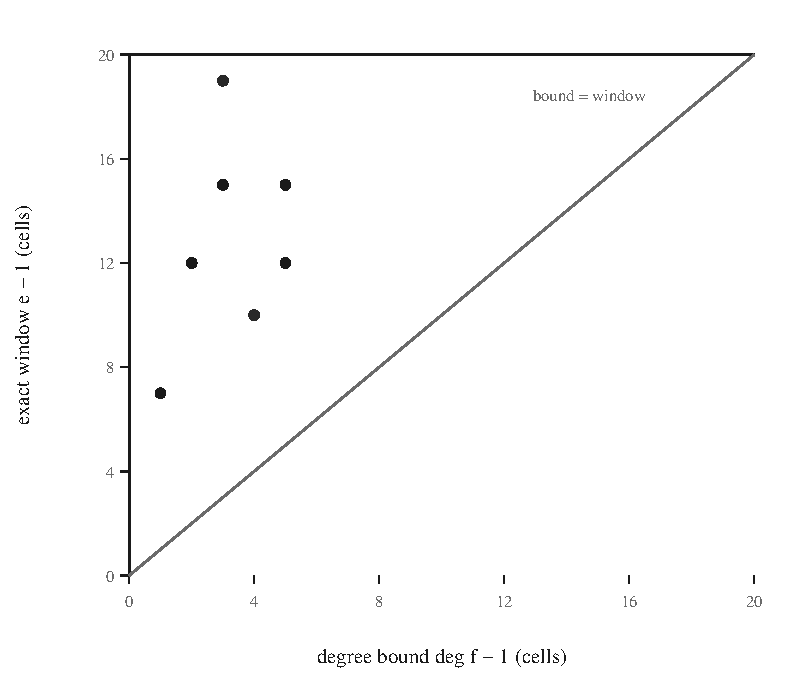
\includegraphics[width=0.8\linewidth]{figures/fig_scatter.pdf}
\caption{Exact window $e-1$ against the degree bound $\deg f-1$ for all branches over $\F_3$ with $2\le n\le20$ and $\gcd(n,3)=1$. Points above the diagonal are branches for which the degree criterion is not sharp; the diagonal is drawn for reference.\label{fig:scatter}}
\end{figure}

\subsection{Collision sets and windows}

Theorem \ref{sharp} was checked against the directly computed syndrome map for $1\,970$ branches: for each branch the set of differences $\delta$ with $\Sigma(\alpha)=\Sigma(\alpha+\delta)$ for some $\alpha$ was compared with the set of multiples of $e$, and the two sets coincided in every case. The injectivity boundary was checked separately: for $540$ combinations of branch and split $(a_l,a_r)$ with $a_l+a_r=e-1$ the map was injective, and with $a_l+a_r=e$ it was not. Theorem \ref{fused} was checked on $32$ triples of branches drawn from eight pairs, and Theorem \ref{hybrid} on $123$ branch-family combinations, including the boundary case $y=\deg f-1$. Proposition \ref{joint} and the general-residue statement of Appendix B were checked on $708$ combinations of branch and marker residue. In each case the computed collision set matched the predicted one exactly.


\subsection{Fusion, relaxation and the proper-$D$ constraint}

The comparison is made concrete by Table~\ref{tab:fusion}, which lists ring codes assembled from three explicit branches. In every row the fused period equals the best single period, as Theorem \ref{nogain} predicts, and the two no-go lengths are those of Example \ref{nogo}. The table also makes the point of Theorem \ref{nogain} concrete: the ring construction adds quantum symbols ($K$ exceeds what the best single component would carry) but not synchronization.


\begin{table}[t]
\centering
\caption{Ring codes from three explicit branches: periods, fused period, best single period and parameters. For $(3,10)$ and $(7,10)$ no branch exists.\label{tab:fusion}}
\small
\begin{tabular}{rrcccccc}
\toprule
$q$ & $n$ & $(e_1,e_2,e_3)$ & $e_R$ & best single & $N$ & $K$ & window \\
3 & 8 & $(8,8,8)$ & 8 & 8 & 24 & 12 & 7 \\
3 & 13 & $(13,13,13)$ & 13 & 13 & 39 & 21 & 12 \\
5 & 8 & $(4,4,8)$ & 8 & 8 & 24 & 16 & 7 \\
5 & 12 & $(4,4,12)$ & 12 & 12 & 36 & 28 & 11 \\
7 & 6 & $(3,3,6)$ & 6 & 6 & 18 & 12 & 5 \\
7 & 15 & $(3,3,15)$ & 15 & 15 & 45 & 33 & 14 \\
11 & 5 & $(5,5,5)$ & 5 & 5 & 15 & 9 & 4 \\
13 & 6 & $(3,3,6)$ & 6 & 6 & 18 & 12 & 5 \\
3 & 10 & no branch & --- & --- & --- & --- & --- \\
7 & 10 & no branch & --- & --- & --- & --- & --- \\
\bottomrule
\end{tabular}

\smallskip
\parbox{\linewidth}{\footnotesize Each row was realised by an explicit triple of branches whose component dimensions reproduce the listed $K$; the window is $e_R-1$ cells.}
\end{table}

Table~\ref{tab:relax} lists the relaxation families with the largest factors in the enumeration of Remark \ref{relax}. Figure~\ref{fig:relax} shows the distribution of the factor over all $118$ pairs: most pairs gain nothing, but a substantial minority does, and the tail reaches $12$ within the stated cutoff.


\begin{table}[t]
\centering
\caption{Relaxation families with linear branches ($n\mid q-1$): the seven pairs with factor at least $6$ in the enumeration of Remark \ref{relax}.\label{tab:relax}}
\small
\begin{tabular}{rrccc}
\toprule
$q$ & $n$ & component periods $(m_1,m_2,m_3)$ & $e_R$ & $n/\max_im_i$ \\
61 & 60 & $(3,4,5)$ & 60 & 12 \\
73 & 72 & $(3,8,9)$ & 72 & 8 \\
89 & 88 & $(4,8,11)$ & 88 & 8 \\
71 & 70 & $(5,7,10)$ & 70 & 7 \\
43 & 42 & $(3,6,7)$ & 42 & 6 \\
67 & 66 & $(3,6,11)$ & 66 & 6 \\
79 & 78 & $(3,6,13)$ & 78 & 6 \\
\bottomrule
\end{tabular}

\smallskip
\parbox{\linewidth}{\footnotesize For $q\le101$ all $118$ pairs and their selected triples are given in the accompanying data set; $38$ have factor $>1$. Ties in minimising the largest period are broken lexicographically. The selected branches are linear, $C_i=\gen{x-a_i}\subsetneq\F_q^n$, so $D_i=\F_q^n$ and $d_X=1$ in every row.}
\end{table}

\begin{figure}[t]
\centering
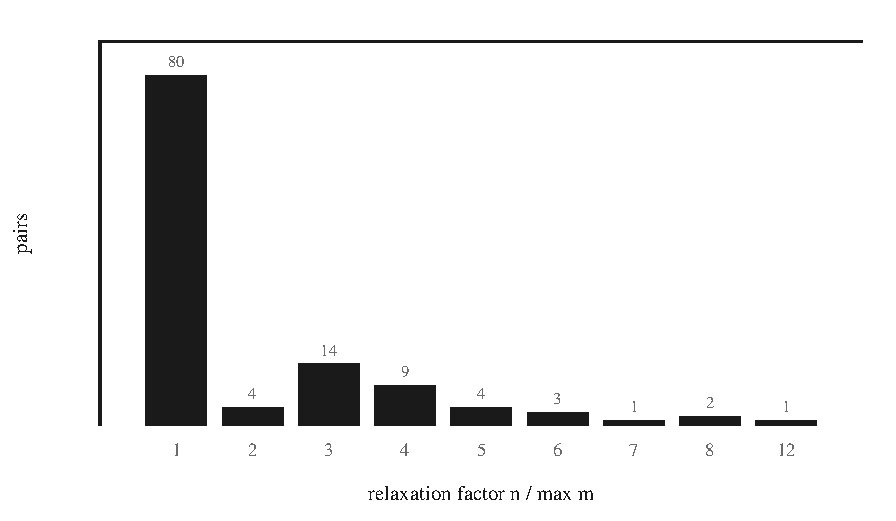
\includegraphics[width=0.8\linewidth]{figures/fig_relax.pdf}
\caption{Distribution of the relaxation factor $n/\max_im_i$ over the $118$ pairs of Remark \ref{relax}.\label{fig:relax}}
\end{figure}

Imposing the constraint that $D$ be proper restricts $d_X\ge2$ by Remark \ref{properD} and reduces the list to $27$ pairs, tabulated in Table~\ref{tab:dconstr}. Every one of them still admits a triple with fused period $n$, so the negative result of Theorem \ref{nogain} is not an artefact of degenerate branches; the question left open is the behaviour for $d_X\ge4$.


\begin{table}[t]
\centering
\caption{All $27$ pairs for which a branch with proper $D$ exists, with the attainable periods $E$ and a witness triple whose least common multiple is $n$.\label{tab:dconstr}}
\small
\begin{tabular}{rrlr}
\toprule
$q$ & $n$ & attainable periods $E$ & witness \\
3 & 13 & $\{13\}$ & $(13,13,13)$ \\
3 & 16 & $\{8,16\}$ & $(8,8,16)$ \\
5 & 8 & $\{4,8\}$ & $(4,4,8)$ \\
5 & 12 & $\{4,12\}$ & $(4,4,12)$ \\
5 & 16 & $\{4,8,16\}$ & $(4,4,16)$ \\
7 & 6 & $\{3,6\}$ & $(3,3,6)$ \\
7 & 9 & $\{3,9\}$ & $(3,3,9)$ \\
7 & 12 & $\{3,6,12\}$ & $(3,3,12)$ \\
7 & 15 & $\{3,15\}$ & $(3,3,15)$ \\
7 & 16 & $\{16\}$ & $(16,16,16)$ \\
7 & 18 & $\{3,6,9,18\}$ & $(3,6,9)$ \\
7 & 19 & $\{19\}$ & $(19,19,19)$ \\
11 & 5 & $\{5\}$ & $(5,5,5)$ \\
11 & 10 & $\{5,10\}$ & $(5,5,10)$ \\
11 & 14 & $\{7,14\}$ & $(7,7,14)$ \\
11 & 15 & $\{5,15\}$ & $(5,5,15)$ \\
11 & 16 & $\{8,16\}$ & $(8,8,16)$ \\
11 & 19 & $\{19\}$ & $(19,19,19)$ \\
11 & 20 & $\{5,10,20\}$ & $(5,5,20)$ \\
13 & 6 & $\{3,6\}$ & $(3,3,6)$ \\
13 & 8 & $\{4,8\}$ & $(4,4,8)$ \\
13 & 9 & $\{3,9\}$ & $(3,3,9)$ \\
13 & 12 & $\{3,4,6,12\}$ & $(3,3,4)$ \\
13 & 15 & $\{3,15\}$ & $(3,3,15)$ \\
13 & 16 & $\{4,8,16\}$ & $(4,4,16)$ \\
13 & 18 & $\{3,6,9,18\}$ & $(3,6,9)$ \\
13 & 20 & $\{4,20\}$ & $(4,4,20)$ \\
\bottomrule
\end{tabular}

\smallskip
\parbox{\linewidth}{\footnotesize $E$ lists all periods $\ord_x(f)$ realised by branches with proper $D$ for that pair; a single branch already attains $\max E=n$ in every row. The other $54$ pairs of the census admit no such branch.}
\end{table}

\subsection{The flagship code}

For the code of Example \ref{flagship} the stabilizer group was constructed explicitly and its generators were verified to commute pairwise; the $X$-type part and the $Z$-type part each have rank $18$ over $\F_3$, giving $K=39-2\cdot18=3$ in agreement with @eq:flagship. The distances $d_Z=4$ and $d_X=3$ were obtained by enumerating all $2\,187$ and $59\,049$ words of $C$ and $D$; no word of $D\setminus C^\perp$ has weight below $3$, and the minimum is attained. The marker cascade of Table~\ref{tab:alloc} was verified by computing the collision sets directly from equation \eqref{eq:collision} for each allocation, not from Theorem \ref{hybrid}.


\subsection{Complexity}

The computations have three layers with different costs. Factoring $x^n-1$ by distinct-degree decomposition and Cantor--Zassenhaus splitting costs $O(n^2\log n)$ field operations with schoolbook polynomial arithmetic, plus the cost of the randomised splitting. Computing $e=\ord_x(f)$ for one branch costs $O(n^2\log^2 n)$ in the worst case, since $e\mid n$, the exponent is found by dividing $n$ by its prime factors, and each of the $O(\log n)$ trials requires a modular exponentiation costing $O(n^2\log n)$. Enumerating all branches of a pair costs $5^m-3^m$ steps for $m$ reciprocal factor pairs, which is exponential in $m$; in the census $m\le6$, so no pair required more than $14\,896$ enumerations. Brute-force collision sets cost $O(n^2)$ syndrome comparisons per branch and were used only where the exhaustive check was the point; the criterion of Theorem \ref{sharp} computes the same set in $O(n)$ after $e$ is known. Message-collision tests cost $O(n q^{y})$ reductions modulo $f$, which is why the message tables are confined to small $y$. Distance computations require enumerating $q^{k}$ words and were therefore restricted to codes with $q^{k}\le6\times10^{4}$.


Measured on one core of the verification environment, the complete core suite of eighteen theorem checks, which includes $1\,970$ branch collision sets and $540$ window splittings, runs in $25.1$ s, and the entire census of $20\,724$ branches over $81$ pairs runs in $0.17$ s. These figures describe construction-time algebra; they say nothing about the cost of decoding a received block, which is not analysed here.


\section{Discussion and limitations}\label{sec:discussion-and-limitations}

The results above are exact within their model, and the model is narrow. It is worth being specific about what the narrowness excludes, because the phrase "synchronizable code" can suggest a physical capability that the theorems do not deliver.


\emph{Exact syndromes.} Assumption (A2) is the substantive restriction. Theorem \ref{sharp} characterises the injectivity of an idealised syndrome map; a physical receiver measures syndromes through a noisy circuit, and errors in that circuit can move the observed syndrome to a value belonging to a different offset. The analysis here neither bounds the resulting error probability nor designs a decoder that tolerates it. A treatment of this question would need to model the syndrome extraction explicitly and to combine the offset estimate with the physical-error correction, which is a different problem from the one solved here.


\emph{Whole-cell offsets.} Misalignments by one or two qudits, which would displace the three components relative to each other, are excluded by construction. The interleaving of Section 3 is what makes the components share an offset, and it is also what forbids offsets that are not multiples of three. A construction that corrects single-qudit offsets would need either a different lift or a nested structure within each component, and we do not propose one.


\emph{Prime fields.} The algebra of Sections 2--4 uses only that $\F_q$ is a field of odd characteristic and that $\gcd(n,q)=1$; the restriction to prime $q$ is a restriction of the computations, not of the theory. Extending the enumerations to prime powers would require field arithmetic over $\F_{p^m}$ and would not change any of the proofs.


\emph{Distances.} The distance statement of Proposition \ref{params} is combinatorial and was evaluated only for small codes, by enumeration. No asymptotic distance analysis is attempted, and the constructions are not compared with the best known quantum codes of comparable length; such a comparison would require either bounds that do not need enumeration or a much larger computational budget.


\emph{Novelty.} The individual ingredients of this paper are known. Ring decompositions of the type @eq:decomp and the idempotents @eq:idem are standard in the construction of quantum codes from cyclic codes over rings \cite{DinhEtAl2021,DinhBagUpadhyay2021}, and synchronizable codes over rings have been constructed before \cite{LiuLiu2021,DaiLiu2022,LiuHuLiu2024}. The order criterion is due to \cite{FujiwaraTonchevWong2013} in the binary case and is used in the $q$-ary literature \cite{XieYangYuan2016,LuoMa2018}. Converse statements, that a window larger than the order bound cannot exist, are also not new in themselves: they follow from the multiplicativity of the order and are implicit wherever the order is described as the period of the marker, for instance in \cite{FujiwaraTonchevWong2013}. Hybrid synchronizable codes, including the trade-offs between synchronization, gauge degrees of freedom and classical capacity, are the subject of \cite{TansuwannontNemec2026}. What we have not found in the literature is the combination used here as a design tool: the exact collision set, applied uniformly across a ring decomposition to show that the degree criterion is never sharp for dual-containing branches, that three components cannot fuse to a period beyond $n$, and that the fusion nevertheless buys a quantifiable relaxation of the per-component period. Which parts of this are genuinely new, as opposed to implicit in the order literature, we cannot settle from the sources available to us. In particular we could not obtain the full text of \cite{LiZhu2022}, whose title and abstract indicate the closest overlap, so we cannot exclude that part of the ring construction is anticipated there. This is a limitation of our search, not a claim about that paper, and it is the reason the contribution is stated as a combination rather than as an individual theorem.


\emph{Optimality.} No optimality is claimed. The thresholds are exact for the codes considered, but the codes are not shown to be optimal in any sense, and the relaxation families of Remark \ref{relax} have $d_X=1$, which makes them poor choices for Pauli-error protection even though their synchronization parameters are excellent.


\emph{Question \ref{distance}.} The behaviour of the fused period under a distance constraint $d_X\ge4$ is open in this paper. It is conceivable that the constraint forces every branch to have small order, which would make the relaxation of Remark \ref{relax} unavailable in the regime where it matters most; we did not find a proof either way.


Two positive conclusions survive these caveats. The first is methodological: for design purposes the quantity to compute is $\ord_x(f)$, not $k_D-k_C$, and the difference between the two can be a factor of six in window for a code as small as the one in Example \ref{flagship}. The second is structural: the three-component ring does not enlarge the window, but it does allow the window to be carried by a component whose period is small while the other components carry messages, and it allows the synchronized part of a design to be separated from the parts that are optimized for distance.


\section{Conclusion}\label{sec:conclusion}

We analysed synchronizable hybrid codes obtained from cyclic codes over $R=\F_q[v]/(v^3-v)$ for odd prime $q$, using the idempotent decomposition $R\cong\F_q^3$ and an interleaved lift to $3n$ qudits grouped into cells. Within the idealised model of exact marker syndromes, collision sets, existence and fused thresholds are characterised by proofs, and the numerical statements were confirmed independently.


The undetectable offsets of a branch are exactly the multiples of $e=\ord_x(f)$, so the window is $e-1$ and the known sufficient order condition is also necessary in the ideal model. For every dual-containing branch $\deg f\le e-1$, so the degree-type criterion is never sharp; the census of $20\,724$ branches confirms this, and for the $[13,7,4]\subseteq[13,10,3]$ branch over $\F_3$ the exact window of twelve cells is six times the two cells that the degree criterion certifies.


Branches of length $n$ exist if and only if $-1\notin\gen{q}\bmod n$, and then one of them has period $n$. Three components fuse with period $\lcm(e_1,e_2,e_3)$, which never exceeds $n$ and is already attained by a single component: fusion does not enlarge the window. What it does provide is a relaxation of the per-component requirement, whose factor is bounded by $12$ in the enumeration with $q\le101$ but is unbounded in general, at the cost of a poor $X$-distance.


With message-carrying markers the window is governed by an exact membership criterion, a collision at difference $\delta$ forces $|\delta|+y\ge\deg f$, and the frame can be held by one component while the others transmit. In the ternary example the underlying hybrid code has parameters $[[39,3:9,0,3]]_3$ and four of its nine classical symbol slots can be used for messages at a twelve-cell window and a padded length of $75$ qudits.


The natural continuations are the three that the limitations make visible: a model in which the marker syndrome is noisy and the offset estimate is combined with physical-error correction; offsets by single qudits, which require a different lift; and Question \ref{distance}, the behaviour of the fused period under a distance constraint. A fourth, more speculative direction is to replace the three-component ring by $\F_q[v]/(v^{k+1}-v)$ with $k+1$ components, where Theorem \ref{nogain} applies verbatim but the relaxation and allocation trade-offs change.


\appendix

\section{The sign in the collision criterion}\label{sec:appendix-the-sign-in-the-collision-criterion}

In characteristic two the polynomials $x^\delta b-b'$ and $x^\delta b+b'$ coincide. In odd characteristic a shift by $\delta$ multiplies a codeword polynomial by $x^\delta$, so the collision condition is $f\mid x^\delta b-b'$, and for $b=b'=1$ it reads $f\mid x^\delta-1$. The condition $f\mid x^\delta+1$, obtained with the opposite sign, holds exactly when $x^\delta\equiv-1\pmod f$, which requires $e$ even and $\delta\equiv e/2\pmod e$; its solution set is therefore disjoint from the set of multiples of $e$. Since $e/2$ is never a multiple of $e$, using the wrong sign would produce a collision set of the wrong size and, in the case $e=2$, a window of zero for a branch whose true window is one.


\section{Marker residues that are not coprime to the generator quotient}\label{sec:appendix-marker-residues-that-are-not-coprime-to-the-generator-quotient}

Theorem \ref{sharp} assumes $\gcd(\beta,f)=1$. The general case is not much harder and is useful when the marker is chosen for reasons other than synchronization, for instance to make the message family a subgroup.


\begin{proposition}\label{residue}
Let $g=g_D\beta$ with $\beta$ not identically zero modulo $f$, and put $d=\gcd(\beta,f)$ and $f_0=f/d$. Then $\delta$ is a collision for the marker $g$ if and only if $f_0\mid x^\delta-1$; the collision set is the set of multiples of $\ord_x(f_0)$, and the window is $\ord_x(f_0)-1$. If $\beta\equiv0\pmod f$, that is $g\in C$, every difference is a collision and the window is zero.
\end{proposition}

\textbf{Proof.} By Lemma \ref{collision} with $\beta'=\beta$, a difference $\delta$ is a collision if and only if $f\mid\beta(x^\delta-1)$. Writing $\beta=d b$ and $f=d f_0$ with $\gcd(b,f_0)=1$, this is equivalent to $f_0\mid x^\delta-1$. The order of $x$ modulo $f_0$ is defined because $f_0(0)\neq0$, being a divisor of $f$, and the collision set is the set of its multiples. If $\beta\equiv0$ the condition holds for every $\delta$. $\square$


Proposition \ref{residue} shows that a marker sharing a factor with $f$ keeps a window equal to $\ord_x(f_0)-1$ for the reduced modulus $f_0$, which divides $e$; in particular the window can only decrease, and it does so by the order of the discarded factor. This is the precise sense in which the coprimality hypothesis of Theorem \ref{sharp} is a convenience rather than a restriction on the construction.



\bibliographystyle{amsplain}
\bibliography{References}

\end{document}
